\documentclass{article}
\usepackage[utf8]{inputenc}
\usepackage[margin=1in]{geometry}
\usepackage{soul,color}
\usepackage{amsfonts, amsmath}
\usepackage{bbm}
\usepackage{enumitem}
\usepackage[nobreak=true]{mdframed}
\usepackage{amssymb}
\usepackage{graphicx}

\newcommand{\solution}{\textbf{Solution: }}
\newcommand{\N}{\mathcal{N}}
% \newcommand{\Pbf}{\textbf{P}}
\newcommand{\R}{\mathbb{R}}
\newcommand{\E}{\mathbb{E}}
\newcommand{\Var}{\text{Var}}
\newcommand{\Cov}{\text{Cov}}
\newcommand{\Ell}{\mathcal{L}}
\DeclareMathOperator*{\argmin}{argmin}

\usepackage[utf8]{inputenc}

% Default fixed font does not support bold face
\DeclareFixedFont{\ttb}{T1}{txtt}{bx}{n}{8} % for bold
\DeclareFixedFont{\ttm}{T1}{txtt}{m}{n}{8}  % for normal

% Custom colors
\usepackage{color}
\definecolor{deepblue}{rgb}{0,0,0.5}
\definecolor{deepred}{rgb}{0.6,0,0}
\definecolor{deepgreen}{rgb}{0,0.5,0}

\usepackage{listings}

% Python style for highlighting
\newcommand\pythonstyle{\lstset{
language=Python,
basicstyle=\ttfamily\footnotesize,
otherkeywords={self},             % Add keywords here
keywordstyle=\ttb\color{deepblue},
emph={MyClass,__init__},          % Custom highlighting
emphstyle=\ttb\color{deepred},    % Custom highlighting style
stringstyle=\color{deepgreen},
frame=tb,                         % Any extra options here
showstringspaces=false           % 
}}


% Python environment
\lstnewenvironment{python}[1][]
{
\pythonstyle
\lstset{#1}
}
{}

% Python for external files
\newcommand\pythonexternal[2][]{{
\pythonstyle
\lstinputlisting[#1]{#2}}}

% Python for inline
\newcommand\pythoninline[1]{{\pythonstyle\lstinline!#1!}}

\title{CS189, HW7: Unsupervised}
\author{ Completed by: Matthew Wu}
% \date{January 2017}
\date{}

\begin{document}

\maketitle

\subsection*{1. $k$-means clustering}
The code used to generate the k-means clustered images is in the appendix.\\

\begin{mdframed}
Means for 5 clusters:\\


\includegraphics[]{images/mnist-5-clusters/0.png} 
\includegraphics[]{images/mnist-5-clusters/1.png} 
\includegraphics[]{images/mnist-5-clusters/2.png} 
\includegraphics[]{images/mnist-5-clusters/3.png} 
\includegraphics[]{images/mnist-5-clusters/4.png}
\end{mdframed}

\begin{mdframed}
Means for 10 clusters:\\


\includegraphics[]{images/mnist-10-clusters/0.png} 
\includegraphics[]{images/mnist-10-clusters/1.png} 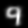
\includegraphics[]{images/mnist-10-clusters/2.png} 
\includegraphics[]{images/mnist-10-clusters/3.png} 
\includegraphics[]{images/mnist-10-clusters/4.png} 
\includegraphics[]{images/mnist-10-clusters/5.png} 
\includegraphics[]{images/mnist-10-clusters/6.png} 
\includegraphics[]{images/mnist-10-clusters/7.png} 
\includegraphics[]{images/mnist-10-clusters/8.png} 
\includegraphics[]{images/mnist-10-clusters/9.png}

\end{mdframed}

\begin{mdframed}
Means for 20 clusters:\\


\includegraphics[]{images/mnist-20-clusters/0.png} 
\includegraphics[]{images/mnist-20-clusters/1.png} 
\includegraphics[]{images/mnist-20-clusters/2.png} 
\includegraphics[]{images/mnist-20-clusters/3.png} 
\includegraphics[]{images/mnist-20-clusters/4.png} 
\includegraphics[]{images/mnist-20-clusters/5.png} 
\includegraphics[]{images/mnist-20-clusters/6.png} 
\includegraphics[]{images/mnist-20-clusters/7.png} 
\includegraphics[]{images/mnist-20-clusters/8.png} 
\includegraphics[]{images/mnist-20-clusters/9.png}


\includegraphics[]{images/mnist-20-clusters/10.png} 
\includegraphics[]{images/mnist-20-clusters/11.png} 
\includegraphics[]{images/mnist-20-clusters/12.png} 
\includegraphics[]{images/mnist-20-clusters/13.png} 
\includegraphics[]{images/mnist-20-clusters/14.png} 
\includegraphics[]{images/mnist-20-clusters/15.png} 
\includegraphics[]{images/mnist-20-clusters/16.png} 
\includegraphics[]{images/mnist-20-clusters/17.png} 
\includegraphics[]{images/mnist-20-clusters/18.png} 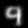
\includegraphics[]{images/mnist-20-clusters/19.png}
\end{mdframed}

With only 5 clusters, obviously not all 10 digits can be separated into clusters. However, 0, 1, 3, and 9 appear to be fairly distinct digits in the space, and the other digits get averaged into the last cluster. Increasing the number of clusters to 10, we still can't identify all the digits, because 1, 9 and 3 are distinctive digits. We pick up on a few more digits like 8 and 7, but the remaining digits are averaged in the last cluster. After we reach 20 clusters, we have enough clusters such that we can see clusters that resemble each digit. Some digits, like 6, are fairly similar to other digits and only appear in one cluster, but other digits that are presumably very distinctive like 0 appear in multiple clusters.

\newpage

\section*{Low-Rank approximation}
The code used to generate the images and graphs in this section is in the appendix.
\begin{enumerate}[label=\alph*)]
\item Low rank approximations of the face image:

\begin{tabular}{|c|c|c|}
\hline
\textbf{Rank-5 Image} & \textbf{Rank-20 Image} & \textbf{Rank-100 Image} \\
\hline
\phantom{} & \phantom{} & \phantom{} \\
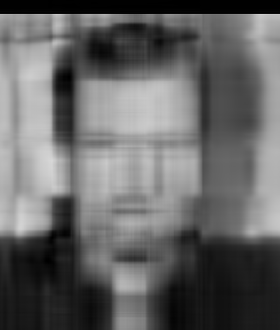
\includegraphics[scale=.45]{images/low-rank_approx/face-5.png} & 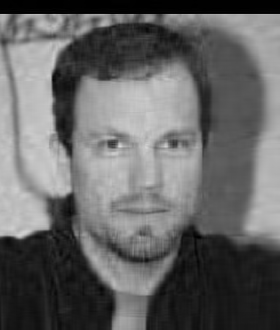
\includegraphics[scale=.45]{images/low-rank_approx/face-20.png} & 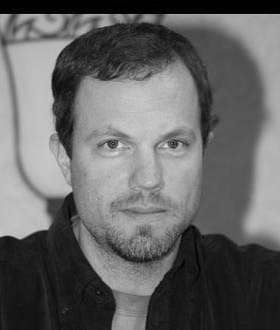
\includegraphics[scale=.45]{images/low-rank_approx/face-100.png} \\
\hline
\end{tabular}
\item
Mean squared error plot:\\
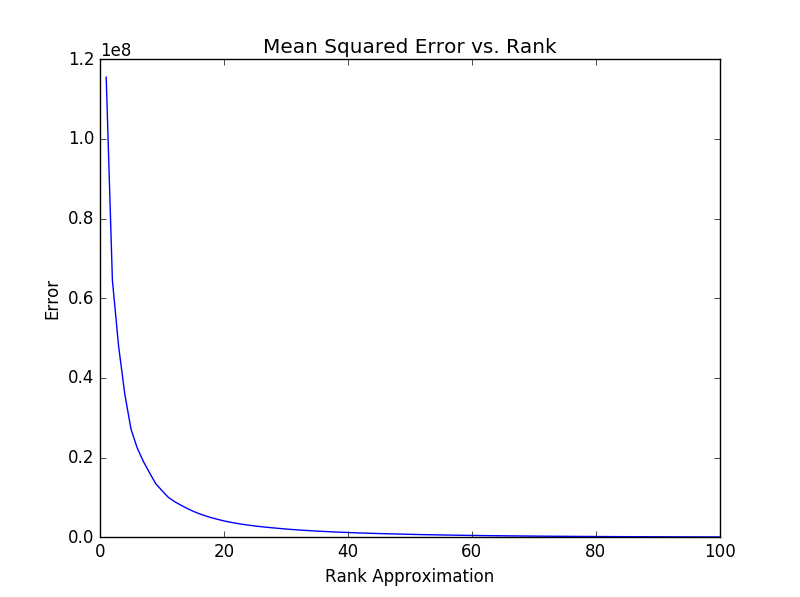
\includegraphics[scale=.7]{images/low-rank-MSE.png}
\newpage
\item Low rank approximations of the sky image:

\begin{tabular}{|c|c|c|}
\hline
\textbf{Rank-5 Image} & \textbf{Rank-20 Image} & \textbf{Rank-100 Image} \\
\hline
\phantom{} & \phantom{} & \phantom{} \\
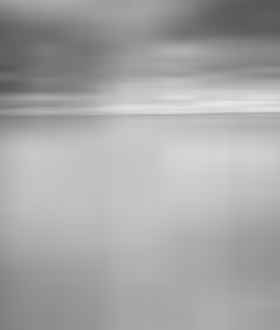
\includegraphics[scale=.45]{images/low-rank_approx/sky-5.png} & 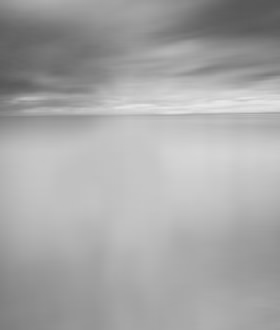
\includegraphics[scale=.45]{images/low-rank_approx/sky-20.png} & 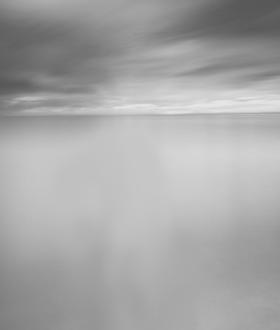
\includegraphics[scale=.45]{images/low-rank_approx/sky-100.png} \\
\hline
\end{tabular}
\item For the face image, at rank 40 it's still grainy. At rank 60, the image is still ever so slightly grainy, but the only real places where the approximation is worse than the original is a slightly blurrier beard and a slightly less smooth shadow edge. At rank 80 I can't perceive any difference from the original image.\\

The sky can already be approximated fairly accurately at rank 5. There's clearly fewer finer details outlining distinct clouds and reflections off the water, but overall, but they're still similar regardless. At rank 20 I can't perceive any difference from the original image.\\

The face requires a higher rank to approximate with more fidelity due to the face's complicated shape. There's a shirt, there's hair, there's ears, there's eyes, there's a beard, etc, and edges around all of these objects, and it's difficult to accurately capture of all these features with high detail with a low rank image. The sky, on the other hand, is a relatively simple image. All there is is the water and the clouds. The only distinctive edge is the horizon, and the details in the water and the clouds are mostly gradients.
\end{enumerate}

\newpage
\section*{Joke Recommender System}
Opt-out

\newpage
\section*{Appendix}
Code for k-means clustering:
\begin{python}
import numpy as np
import scipy.io
import matplotlib.pyplot as plt
import csv
import scipy.misc
import sys
import os
import random

traindatafilename = "hw7_data/mnist_data/images"
data = scipy.io.loadmat(traindatafilename)

images = data['images']

samples = np.transpose(images.reshape((784, 60000)))
samples = samples * 1.0

def k_means(num_clusters, max_iterations = 250):
    #starting_indecies = random.sample(range(60000), num_clusters)

    #k_means++ method of picking starting indexes
    first_index = random.randrange(60000) #Pick starting point
    starting_indecies = [first_index]
    current_sample = samples[first_index]

    distances = np.sum((samples - current_sample)**2, axis=1)

    for i in range(num_clusters - 1):
        #Select a random point via kmeans++ method
        total_distance = np.sum(distances)
        target = np.random.random() * total_distance
        val = 0
        j = 0
        while True:
            val += distances[j]
            if val >= target:
                break
            j += 1
        #Add the new point and update point distances
        starting_indecies.append(j)
        current_sample = samples[j]
        dist_to_new_point = np.sum((samples - current_sample)**2, axis=1)
        distances = np.minimum(distances, dist_to_new_point)

    #Initialize the clusters
    clusters = samples[[starting_indecies]]

    iteration = 0

    #samp_norm_squared = np.sum(samples**2, axis = 1).reshape((60000, 1))
    prev_closest_clusters = None

    #Update loop
    while iteration < max_iterations:
        iteration += 1

        #Find points closest to each cluster
        #||u-v||^2 == u*u + v*v - 2(u*v)
        clust_norm_squared = np.sum(clusters ** 2, axis = 1)
        samp_dot_clust = np.inner(samples, clusters)
        #squared_distance_mat = samp_norm_squared + clust_norm_squared - 2 * samp_dot_clust
        squared_distance_mat = clust_norm_squared - 2 * samp_dot_clust

        #squared_distance_mat:
        #(num_samples, num_clusters) matrix
        #squared_distance_mat[i, j] is the distance between point i and cluster j

        #closest_cluster finds the closest cluster index for each sample point
        closest_clusters = np.argmin(squared_distance_mat, axis=1)

        if iteration > 1:
            if (closest_clusters == prev_closest_clusters).all():
                print("\nConverged")
                break

        prev_closest_clusters = closest_clusters

        #cost = 0
        #Calculate the new cluster centers
        for c in range(num_clusters):
            samples_in_cluster = samples[np.where(closest_clusters == c)]
            new_center = np.sum(samples_in_cluster, axis=0) / samples_in_cluster.shape[0]
            #cost += np.sum((samples_in_cluster - new_center)**2)
            clusters[c] = new_center

        print("\nIteration " + str(iteration))
        #print("Cost: " + str(cost))
        sys.stdout.flush()

    if iteration == max_iterations:
        print("\nMaximum iterations reached")

    #Finished finding cluster centers, Save cluster center images
    directory = 'images/mnist-' + str(num_clusters) + '-clusters/'
    if not os.path.exists(directory):
        os.makedirs(directory)
    for c in range(num_clusters):
        cluster = clusters[c]
        cluster = cluster.reshape((28, 28))
        s = directory + str(c) + '.png'
        scipy.misc.imsave(s, cluster)

#k_means(5)
#k_means(10)
#k_means(20)
\end{python}
\newpage

Code for lowrank images:
\begin{python}
import numpy as np
import scipy.io
import matplotlib.pyplot as plt
import csv
import scipy.misc
import sys

load_directory = 'hw7_data/low-rank_data/'
save_directory = 'images/low-rank_approx/'

np.set_printoptions(threshold=np.inf)

def make_low_rank_image(filename, rank):
    pic_name = filename[:-4]
    picture = scipy.misc.imread(load_directory + filename)
    u, s, v = np.linalg.svd(picture, False)
    sig = np.zeros((s.shape[0], s.shape[0]))
    for i in range(rank):
        sig[i, i] = s[i]

    new_picture = np.dot(np.dot(u, sig), v)
    new_picture = np.clip(new_picture, 0, 255)
    new_picture = (new_picture + .5).astype('uint8')

    scipy.misc.imsave(save_directory + pic_name + '-' +
        str(rank) + '.png', new_picture)

def plot_MSE(filename):
    picture = scipy.misc.imread(load_directory + filename)
    u, s, v = np.linalg.svd(picture, False)
    sig = np.zeros((s.shape[0], s.shape[0]))
    error_array = []
    for i in range(100):
        sig[i, i] = s[i]
        new_picture = np.dot(np.dot(u, sig), v)
        error = np.sum((picture - new_picture) ** 2)
        error_array.append(error)
    rank_array = [i + 1 for i in range(100)]
    plt.plot(rank_array, error_array)
    plt.title("Mean Squared Error vs. Rank")
    plt.ylabel("Error")
    plt.xlabel("Rank Approximation")
    plt.show()

#make_low_rank_image('face.jpg', 5)
#make_low_rank_image('face.jpg', 20)
#make_low_rank_image('face.jpg', 100)

#make_low_rank_image('sky.jpg', 5)
#make_low_rank_image('sky.jpg', 20)
#make_low_rank_image('sky.jpg', 100)

make_low_rank_image('face.jpg', 80)

#plot_MSE('face.jpg')
\end{python}

\end{document}